\documentclass[10pt, a4paper]{article}
\usepackage[utf8]{inputenc}
 
\usepackage[danish]{babel}
\usepackage{blindtext}
\usepackage[hidelinks]{hyperref}
\usepackage{graphicx}
\usepackage{caption}
\usepackage{subcaption}
\usepackage{xcolor}
\usepackage{url}
\usepackage[margin=1in]{geometry}
\usepackage[square,comma,numbers]{natbib}
\usepackage{float}

\begin{document}

\section{Exo-Aider armband update}

This document will give an update on the progress of the data-collection armband in the Exo-Aider project. The development of the armband is currently stalled because of the current COVID-19 situation. 



\subsection{Hardware}
The first revision of the hardware (filters, SPI connections and DAC/ADC) have been debugged and tested through with good results and some changes to the hardware. The next revision of the hardware is already designed and the pin-out of the PCB is in progress. Hopefully the next revision of the hardware will be ready to test when the we get back at the university.  


\subsection{Armband}
To make the armband easy to attach it is being build around a blood pressure armband as shown in \autoref{fig:armband}. This also makes it easier to attach yourself and by that also makes it easier to test by yourself. 

\begin{figure}[htbp]
    \centering
    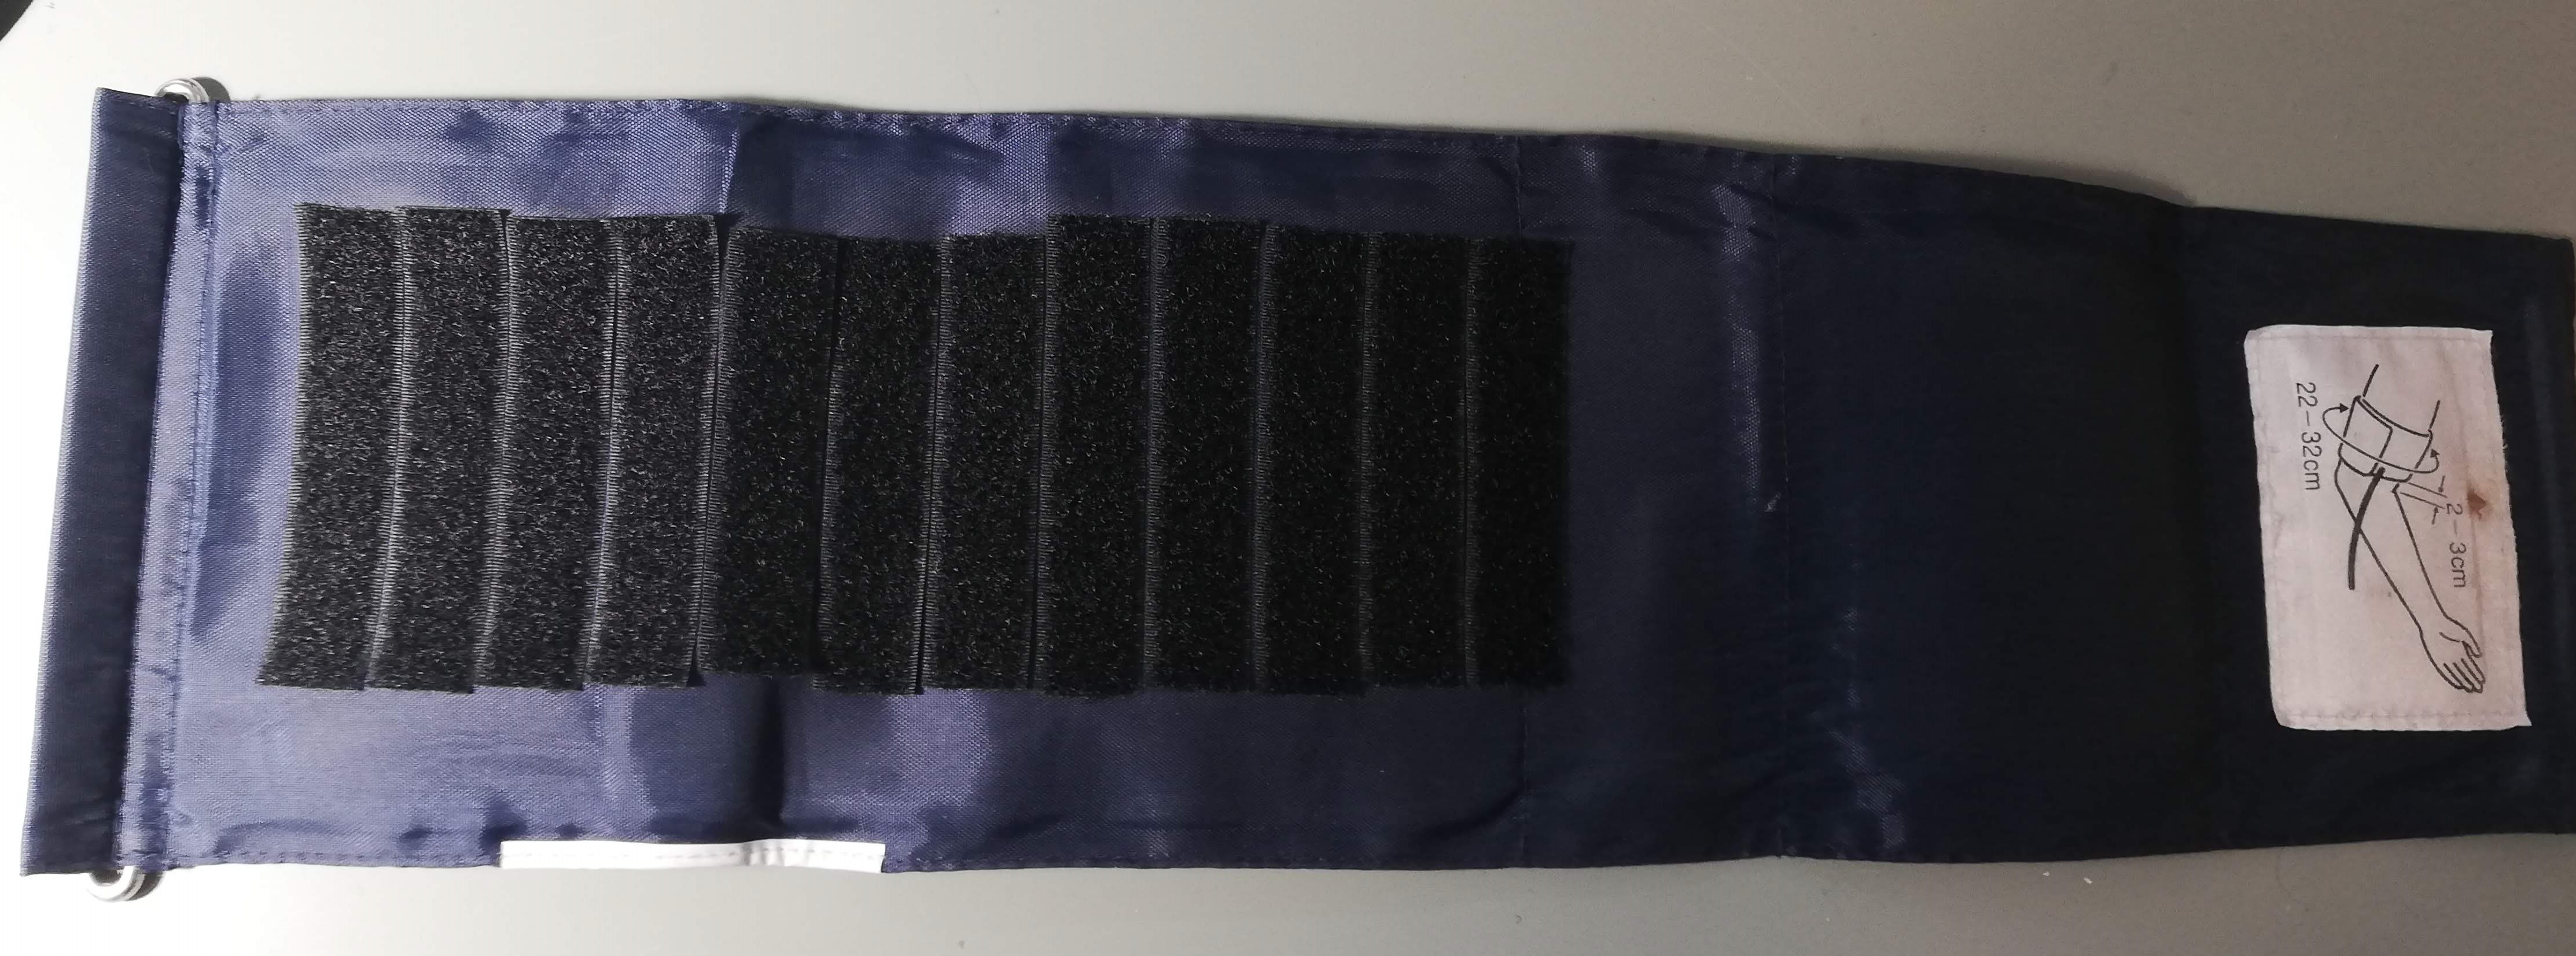
\includegraphics[width=0.8\textwidth]{figures/armband.jpg}
    \caption{Blood pressure armband with Velcro}
    \label{fig:armband}
\end{figure}

The sensors will be build into two modules consisting of four FSR sensors and two sEMG sensors for each module as shown on \autoref{fig:onmodule} which show the concept of the module since the materials for finishing the modules are not available at the moment. 

\begin{figure}[htbp]
    \centering
    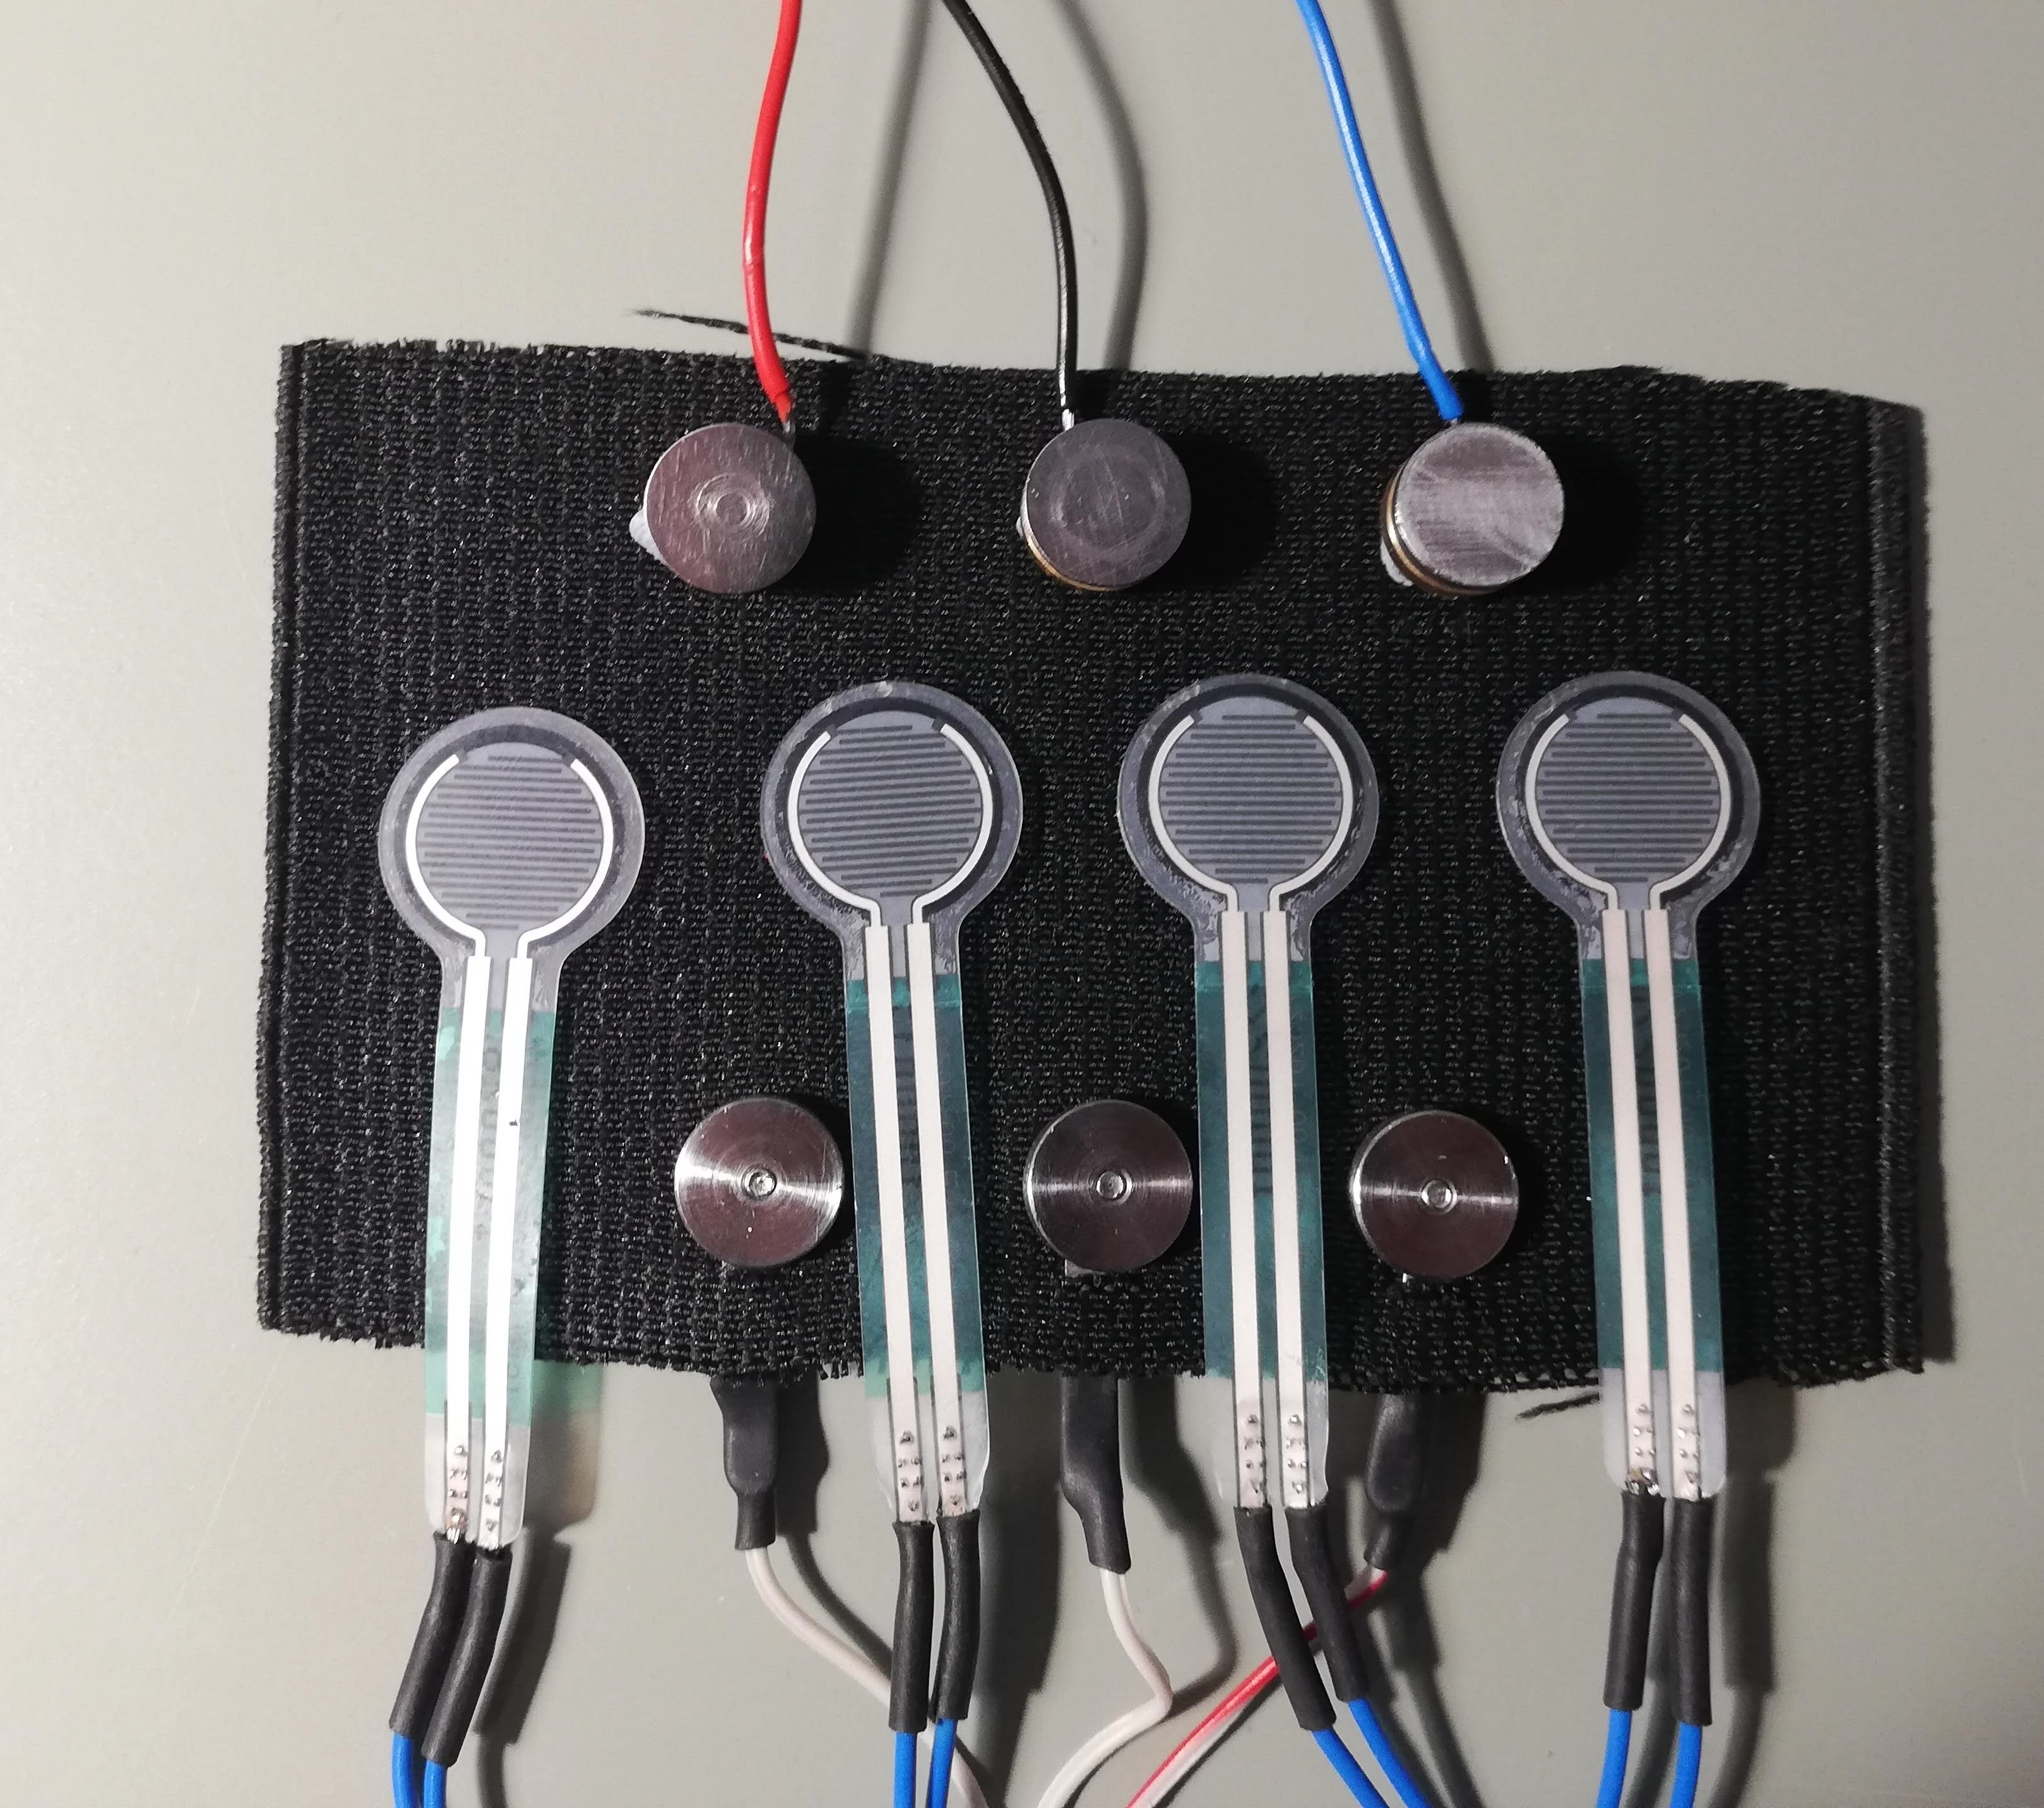
\includegraphics[width=0.4\textwidth]{figures/one_module.jpg}
    \caption{One module consisting of four FSR sensors and two sEMG sensors}
    \label{fig:onmodule}
\end{figure}

By making the armband modular it is possible to move each module around to target the biceps and the triceps of each individual but still keep the same orientation between the sensors in the module. The idea of this is to keep everything as consistent as possible between different people. 


Finally, the armband is almost ready to be combined with the rest of the exoskeleton as soon as the new hardware has been manufactured and tested and the sensors are mounted on the modules.

\end{document}